%
% 公立はこだて未来大学卒業研究中間報告書[全コース対応版]
%
%         ファイル名:"sample.tex"
%
\documentclass[11pt]{jarticle}
%\documentclass[11pt]{ujarticle} %%uplatexを用いる際はこちらを使用
\usepackage{funinfosys}
\usepackage{url}
\usepackage[dvipdfmx]{graphicx}
\author{
    1021077 松本葉太\\指導教員 : 新美礼彦
}
%\course{Information Systems Course}
%\course{Advanced ICT Course} %% 高度ICTコースの場合はこちらを使用
%\course{Information Design Course} %% 情報デザインコースの場合はこちらを使用
\course{Complex Systems Course} %% 複雑系科学コースの場合はこちらを使用
%\course{Intelligent Systems Course} %% 知能システムコースの場合はこちらを使用
\title{社会的要因を用いた株価予測}
\etitle{Predicting Stock Prices Based on Social Factors}
\eauthor{Yota Matsumoto}
\abstract{
	近年,国の政策や金利減少の影響などを受けて株取引が注目を集めている.
	特に現役層といわれる20~40歳の株主が増えている.
	そこで本研究では,従来より会社の言動が以前よりも株価に影響するのかを調べ,
	それをもとに従来の株価予測とは違ったアプローチを取り入れることで
	予測精度の向上を目指す.
	例えば,何らかの不祥事を起こし炎上した企業に対するSNSのポストを分析することで,
	どの程度株価に影響を与えるか予測する.
	他にも,新商品に対するSNSでの事前評判で株価に影響があるかも調べる予定である.
	それぞれ別の業界や規模の会社を対象とすることで,それぞれの特徴があるのかも調べる.
	今回はX(旧Twitter)のポストからSNSのポストデータを収集し,極性感情分析を行う.
	}
\keywords{株, SNS, 極性感情分析}
\eabstract{
	In recent years, stock trading has been attracting a lot of attention due to government policies and declining interest rates. 
	In particular, the number of shareholders aged 20~40, considered the working-age group, has been increasing. 
	Therefore, this study aims to improve the accuracy of forecasts by examining whether a company's words 
	and actions affect stock prices more than before and incorporating a different approach 
	from conventional stock price forecasts based on the results. For example, 
	by analyzing the reaction of social networking services to a company that has been under fire for some scandal, 
	we can predict the extent to which the company's actions will affect its stock price. 
	We also plan to examine the impact on stock prices of the advance publicity of new products on social networking services. 
	By targeting companies in different industries and of different sizes, we will also examine the characteristics of each company. 
	In this study, we will collect SNS reaction data from X (formerly Twitter) posts and conduct a polar sentiment analysis.
}
\ekeywords{Stocks, Social networking, Emotional analysis}
\begin{document}
\maketitle
%\vspace*{-.5cm}

\section{背景と目的}
株価予測をするために使われているデータは,企業の財務状況がまとまっている貸借対照表や損益計算書,
キャッシュフロー計算書などの数値を使うことが多い.
しかし,日本証券協会\cite{syoukengyoukai}によると,ここ数年で個人株主が増え,
保有銘柄数も増えている.また一人当たりの平均株式保有数は減少し,20歳から40歳の
現役層と呼ばれる人々が株式取引に参加し,株式の分散化が進んでいる.
実際に株価を下げ発行枚数を増やす,株式分割をすることで
一般人を株取引を推進し,投資家層の拡大を図る企業もある.
このような状況下では,従来株価に影響しないと考えられていた要素が,より大きく株価に
影響を及ぼす可能性がある.現役層が株式を持つことによって,より多くの人が
会社の言動に注目しているだろう.そこで,本研究ではSNSのポストを調べることで,
株価の予測を補助し,予測精度を上げることや新しい株価に影響を与える要素の発見を目的とする.
\section{複雑系コースにおける本研究の位置づけ}
複雑系コースでは現実世界で起きている事象に対して
数理的にモデル化し分析・適応することや法則性を解明するなどの課題
に取り組むことが求められている\cite{funpolicy}.
本研究では,人間社会で実際に動いているデータである株価とSNSに焦点を当て,
SNSから人々の感情を分析し,株価の予測モデルの改善や今まで考えられていなかった株価に影響を
与える要素や法則性の発見を目的としている為,学部カリキュラム・ポリシー\cite{funpolicy}に沿っている.

\section{関連研究}
従来の予測モデルにSNSデータを使い,予測モデルを向上した先行研究の例としては
\cite{posSNS}がある.この研究ではSNSデータから特徴量を収集し,以前からから使われていた
POSデータと組み合わせて使うことで,以前のPOSデータだけを使用していた時よりも予測精度を
上げることに成功した.\\
 機械学習によるFacebookに基づく株価予測\cite{oikawa}では,調査対象企業の
アカウントに対する「いいね」などのアクション数を参照し,話題指数としていた.
それに機械学習を用いることで翌日の株価の増減を予測をしていた.\\
 ネット炎上が株式市場に与える影響についての研究\cite{enjo}では,炎上した時の
企業の対応によって,株価にどのように影響を与えるのかが調査されている.
\cite{enjo}によると,SNSでの炎上が株価下落の原因になる要素として,企業の対応の有無や
報道の有無,個人株主比率,炎上の内容,企業の規模や元々の注目度,存続年数などがある.
炎上が起きる以前から当期純利益がマイナスであったり,売り上げ率が低いなどの企業にとって
マイナスな要素があると炎上を触発しやすい.また,業界ごとに炎上の起きやすさが違い\cite{enjo}
の調査結果では情報通信産業が最も炎上を起こしやすいとされている.

\section{提案する理論}
SNSを用いた株価予測について説明する.今回はX(旧Twitter)のポストから
データを集める.1年分を集める予定であり,半年を実験用にしもう半分を検証用にする.
対象企業は業界や規模が別々になるように集め,それぞれの特徴や法則性がないか調べる.
データには投稿日時,テキスト(ポスト内容),閲覧数,リプライ数,RT数,引用数,アカウント名
フォロワー数が含まれている.収集データのテキストを極性感情分析し株価予測に使う.
極性感情分析には,事前学習済感情分析モデルであるbert-japanese-finetuned-sentimentと
トークナイザー事前学習済モデルbert-base-japanese-whole-word-maskingを用いる.
トークナイザーとは日本語を分析する際に,文章を意味ごとに分解するもののことである.
このトークナイザーは形態素分析という手法で文章を分解している.
これらのモデルを使い,ポスト内容をネガティブ,ポジィティブ,ニュートラルの三つの
感情に分ける.1日ごとに極性感情分析の結果を集計,スコアする.また,\cite{oikawa}のように
いいね数,RT数,リプライ数,閲覧数などを使い同じ一つのポストでも,話題指数による
重さ付けをする.
これらの情報をもとに株価予測モデルを作る.株価予測モデルを作る際は\cite{posSNS}のように
従来のモデルに補助する形で今回のデータを使い,精度の向上を目指す.
予測モデルを作る際は実際の出来事が株価に影響を与えるのに時間差があることを考慮する.

\section{実験と評価}
企業はカドカワ(9468)を対象にX(旧Twittertwitter)にて検索ワードで「kadokawa」で検索し,45785件のポスト情報
を集めた.期間は2024年4月23日~2024年10月25日であり,返信やリンクがついているポストは
広告や告知である可能性が多いため除外した.集めたデータを事前学習モデルbert-japanese-finetuned-sentimentと
トークナイザー事前学習済モデルbert-base-japanese-whole-word-maskingで極性感情分析し,
POSITIVE,NEGATIVE,NEUTRALの3つの感情に分類した.POSITIVE,NEGATIVE,NEUTRALを
それぞれ1,-1,0とした.それらを1日ごとに和をとって集計し,
株価と図にした(図\ref{fig:KadvsLabel}).
\begin{figure}[htbp]
	\centering
	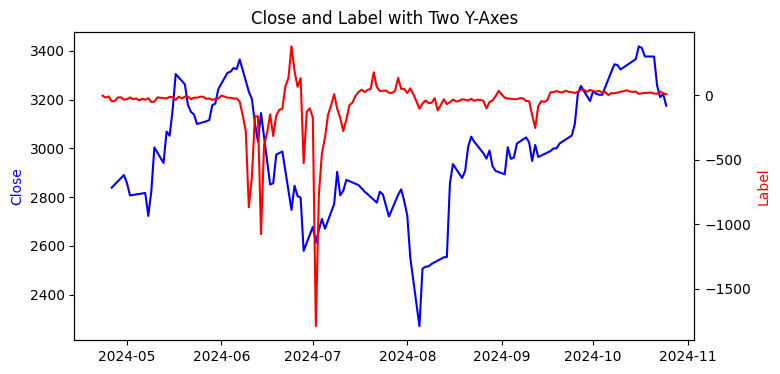
\includegraphics[scale=0.4]{image/KadvsLabel.png}
	
	\caption{Xのポストと株価}
	\label{fig:KadvsLabel}
\end{figure}
\begin{figure}[htbp]
	\centering
	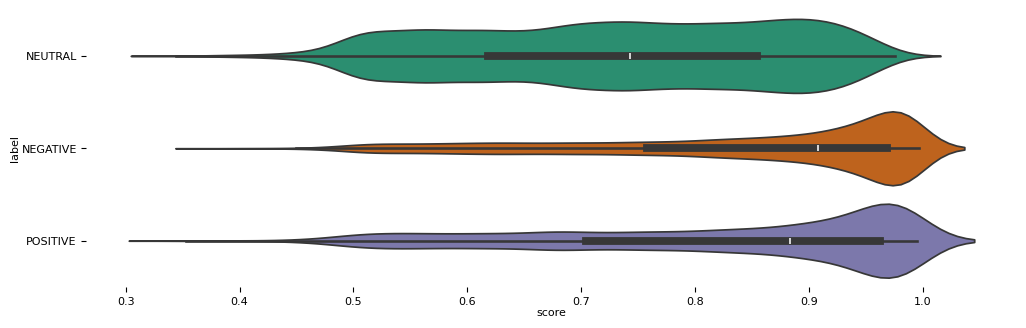
\includegraphics[scale=0.3]{image/score.png}
	
	\caption{Xのポストと株価}
	\label{fig:score}
\end{figure}
青のグラフがカドカワの株価,赤のグラフがXでのポストである.
また,2つの株価はその日の最後の株価である終値を採用した.
感情の分類の信頼度は,学習モデルに備え付けられていたものを使用\ref{fig:score}.
数値が高いほど信頼度が高いことを示す.
POSITIVE,NEUTRALは,1.0の方にグラフが偏っており問題はない.
NEGATIVEだけが0.5あたりの信頼度のものが多く,本来POSITIVEに分類されるべき
ものがNEGATIVEに分類されていないか,少し不安が残るものとなった.
実際はNEGATIVEの判定が特に多かった6月14日と7月2日周辺は
ネットニュースなどになるほど話題になっており,明らかなところは外していないことが分かった.

\section{考察}
図\ref{fig:KadvsLabel}より,実験を踏まえてわかったことは,炎上が起こるとNEGATIVEの判定のポストが多くなり,
株価下落に大きな影響を与えることだ.6月12日の炎上から少し遅れて株価が下落している.これは想定通りの動きとなった.
7月2日の炎上では,株価は炎上が起きるより先に株価が暴落している.このことから,この炎上は株価に関係ない,
もしくは暴落していることについてのポストと予想できる.その後1か月後に暴落があるがあまりにも期間が開いている為
関連性が薄い.そこで,\ref{fig:kadokawa}を見ると日経平均株価の影響だとわかる.
この図は見やすくするために平均0分散1の標準化を施した.


一方,POSITIVEのポストが多いとき株価が上がるかは
わからない.図\ref{fig:kpositive}は,1日ごとのPOSITIVEのポスト数の合計である.
\begin{figure}[htbp]
	\centering
	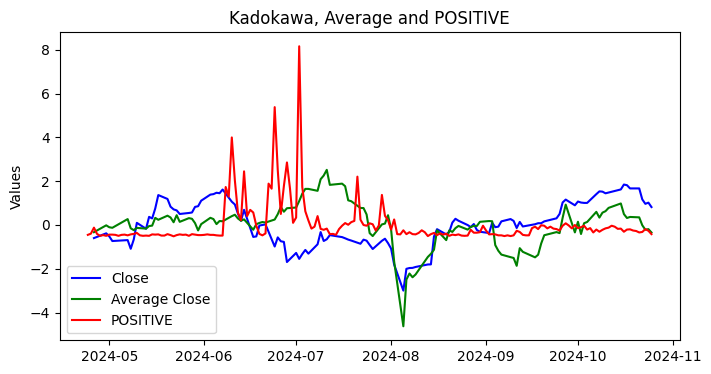
\includegraphics[scale=0.35]{image/k_positive.png}
	
	\caption{POSITIVEポスト数}
	\label{fig:kpositive}
\end{figure}

NEGATIVEのポスト数が多い日であっても,少なからずPOSITIVEのポストがあるが,
今回はNEGATIVEの方が影響度も数も大きく,株価暴落に至ったことがわかる.
しかし,いいね数などの指数をつかえばポスト数が少なくとも影響度をより詳しく
調べられる可能性がある.
\begin{figure}[h]
	\centering
	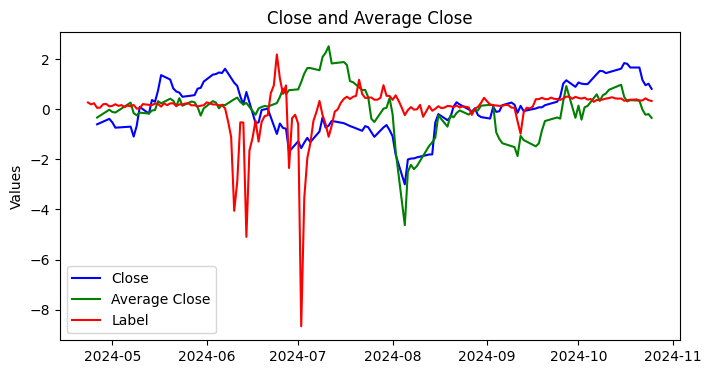
\includegraphics[scale=0.35]{image/kadokawa.png}
	
	\caption{カドカワの株価と日経平均株価とXのポスト}
	\label{fig:kadokawa}
\end{figure}
もう一度,図\ref{fig:kadokawa}を見ると,6月14日の炎上の後,POSITIVEのポストが多くなっているが,日経平均株価も
上がっている為,どちらの影響でカドカワの株価が上がっているか不明である.
その他8月入ってすぐのところではPOSITIVEのポストが多いのにもかかわらず
日経平均株価に影響されカドカワの株価は下落しているところや,NEUTRALのポストが多い
9月以降も基本的に日経平均株価に沿って変動しているように見える.このことから
日経平均株価の影響を踏まえたうえで,Xのポストがどの程度株価に影響しているか見定め
株価予測モデルを構築しなくてはならない.また,企業によって日経平均株価の影響を
受ける度合いが変わっている可能性や為替などの他の考えうる影響が大きい要素にも注意して
他の企業についても調査していく必要がある.

\section{結言}
実験を通して,SNSのポストから株価の予測ができるのではないかという仮説の一部を検証することができた.
今後の展望1つ目はいいね数やれプライ数などからそのポストの影響度を計り,重み付けすることで
精度の向上を目指す.またこれにより,今回のようにポスト数では負けているPOSITIVEの
ポストの影響度を調べられるようになる可能性がある.
2つ目はより多くの企業,業界を分析しそれぞれの特徴を調査することや
今回わからなかったSNSのPOSITIVEなポストの株価に対する影響度を調べることである.
3つ目は実験から得たデータを使い,株価予測モデルの精度向上をすることである.
\begin{thebibliography}{99}
\bibitem{syoukengyoukai}
	日本証券業協会,「個人株主の動向について」,  9, 21, 2022.
 %入手先:https://www.jsda.or.jp/shiryoshitsu/toukei/2022kozinkabunusidoukou.pdf

\bibitem{funpolicy}
	公立はこだて未来大学,	学部カリキュラム・ポリシー,  31, 10, 2024.
	%https://www.fun.ac.jp/curriculum-policy
\bibitem{posSNS}
	西口 真央, 鳥海 不二夫, 河尻 耕太郎, 吉田 光男, 
	小売店POSデータおよびSNSデータを用いた缶ビールの需要予測, 2024年度人工知能学会全国大会 4ページ, 2024.
\bibitem{oikawa}
	及川 健一郎, 堀田 政二, 
	機械学習によるFacebookに基づく株価予測(若葉研究者の集い3,サマーセミナー2014~未来を拓くビジョン技術~), 映像情報メディア学会技術報告, 39-40, 2014.
\bibitem{enjo}
	武田 史子, 森 継哉, ネット炎上が株式市場に与える影響についての研究, 30, 7, 2020.

\end{thebibliography}
\end{document}
%
%
% EOF 
